\documentclass[10pt,twocolumn,letterpaper]{article}

\usepackage{cvpr}
\usepackage{times}
\usepackage{epsfig}
\usepackage{graphicx}
\usepackage{amsmath}
\usepackage{amssymb}

% Include other packages here, before hyperref.

% If you comment hyperref and then uncomment it, you should delete
% egpaper.aux before re-running latex.  (Or just hit 'q' on the first latex
% run, let it finish, and you should be clear).
\usepackage[pagebackref=true,breaklinks=true,letterpaper=true,colorlinks,bookmarks=false]{hyperref}


\cvprfinalcopy % *** Uncomment this line for the final submission

\def\cvprPaperID{****} % *** Enter the CVPR Paper ID here
\def\httilde{\mbox{\tt\raisebox{-.5ex}{\symbol{126}}}}

% Pages are numbered in submission mode, and unnumbered in camera-ready
\ifcvprfinal\pagestyle{empty}\fi
\begin{document}

%%%%%%%%% TITLE
\title{Low-cost Optical Tracking System using Wii Remote}

\author{Wei Zhang, Yi Gong\\
Department of Computer Science\\
University of California, Santa Barbara\\
{\tt\small wei, ygong@cs.ucsb.edu}\\
% For a paper whose authors are all at the same institution,
% omit the following lines up until the closing ``}''.
% Additional authors and addresses can be added with ``\and'',
% just like the second author.
% To save space, use either the email address or home page, not both
%\and
%Second Author\\
%Institution2\\
%First line of institution2 address\\
%{\small\url{http://www.cs.ucsb.edu/~wei}}
}

\maketitle
\thispagestyle{empty}

%%%%%%%%% ABSTRACT
\begin{abstract}
In this project, we proposed a low-cost 3D position tracking system using 
Wii remote controller and IR markers. 
Wii is a very popular console for home entertainment. 
The Wii Remote controller brings revolutionary HCI technologies
to real world and inspires many new applications. However, most of
them only uses the basic functionalities but not exert Wii's full potential.
This work is distinguished from exist
tracking systems by some key features. The first is we exploit the 
multi-view capability of the low-cost Wii remote controller, 
which contains an IR camera and on-board
hardware for signal detection, so that provides the possibility to create
further exciting interactive applications with mininum cost. 
The second is we hide the complexity of computer vision 
since our users may not be vision professionals. 
Currently we have built 
a prototype system and implemented basic multi-view geometry algorithms, 
the final goal of this project is to provide this as an opensource library for other 
Wii developers to create their interactive applications.
\end{abstract}
%-------------------------------------------------------------------------
%%%%%%%%% BODY TEXT
\section{Introduction}
Optical tracking system is a well studied area in the past decades, 
many commercial systems are available in the market. However, most of them 
are complicated and very expensive, built only for professionals.

The Nentindo Wii console has a built-in IR sensor in its remote
controller, with on-board hardware processing capability to track
up to four IR markers simultaneously. This give us the possibility
to build the cheapest motion capture system ever, 
and if consider that Wii has
already been sold to over 20M families, 
our system will only cost them only a few IR markers. 
Such kind of low-cost and tiny motion capture system can be used as a basis 
to build many new applications for home interactive entertainment.

Several interesting application of Wii remote has been developed 
and produce huge impact. The most famous ones are the head tracking
and multi-touch whiteboard developed by Johnny at CMU\cite{JohnnyVR} \cite{JohnnyTouch}.
However, all of current applications only use a single Wii remote for 
its built-in 2D tracking capability.

In our project we are going to build a 3D tracking system using two Wii
remote, this is a classic 3D reconstruction from multiple view problem 
which has been explored by many researchers. For the 2 view cases, 
a lot of studies have been made on the fundamental 
matrix and calibrated or uncalibrated image marching
\cite{luong95},\cite{Higgins87} \cite{Zhang95}~\cite{Hartley95}. 
\cite{Hartley03} is also a good book that cover these issues. 
In our method, we will calibrate our camera by \cite{Zhang00}'s 
algorithm first, then calculate the fundamental matrix 
and reconstruct 3D refer to \cite{Faugeras92}.

In our scenario, user are allowed to place two cameras at anywhere he like,
as long as the markers are visible. So at first the system need to calibrate 
the cameras for their extrinsic and intrinsic parameters. In order
to simplify this process we build a calibration board which has 4 markers
attached on a square with known positions. During the initialization, 
the system detect 
these four points and use the CalibrateCamera2 function in OpenCV to find out 
necessary parameters about cameras.

After the camera's intrinsic and extrinsic parameters are known, the system
is ready to track. There are mainly two problems here. 
The first one is to find the coorespondency 
between object points from different views.
Once this spatial coorespondency is determined then 
inhomogenous linear triangulation method can be applied to reconstruct
the points in 3D space. The second problem involves
matching two sets of 3D points representing detected
markers at two consecutive frames, respectively, thus finally
provide the trajectory of tracking objects.

The rest of the article is arranged as follows: In section 2 we introduce the design
of hardware and software platform that our algorithms are running on, then section 3
provides the details of the camera calibration, 
temporal and spatial coorespondency algorithms. In section 4 we provides a set of
experiment results and discuss the performance of our system and algorithms.

%------------------------------------------------------------------------

%------------------------------------------------------------------------

\section{Platform}
Furthermore, we hope our solution to this problem can become 
an open-source library to help developers building interactive 
applications using Wii remote.
%-------------------------------------------------------------------------
\subsection{Wii Remote}
Wii remote is Wii's main input device. It contains a 1024x768 infrared camera with 
built-in hardware on-board processing to provide 
tracking of up to 4 points (e.g. IR led lights) at 100Hz, 
and it also contains a +/-3g 8-bit 3-axis accelerometer 
which also operating at 100Hz.

Wii remote can be connected to the console 
or PC via bluetooth, this feature gives us the opportunity 
to explore other applications for this hardware rather 
than gaming. 
It uses the standard Bluetooth HID protocol to 
communicate with the host, which is directly based upon 
the USB HID standard, so it will appear as a 
standard input device to any Bluetooth host. 
However, the Wiimote does not make use of the standard 
data types and HID descriptor, and only describes 
its report format length, leaving the actual contents undefined, 
which makes it useless with standard HID drivers. 
The Wiimote actually uses a fairly complex set of operations, 
transmitted through HID Output reports, and returns a number 
of different data packets through its Input reports, 
which contain the data from its peripherals.

Wii community has been succeeded in trying 
to discover the control and communication with the Wii remote, 
there are several opensource software beed released.
In this project, we use our modified driver based the 
opensource Wiimote library to drive multiple input devices.
%-------------------------------------------------------------------------
\subsection{IR Markers and Calibration}
The most sensitive wavelength for Wii remote is between 800 and 950 nm.
The LEDs that we use are Vishay TSAL6400/6200s running at 100mA.

Our IR markers are very simple and easy to build. 
Each IR marker is actually an AA battery and an small IR LED
connected by a switch. 

The calibration board is a plane board 
with 4 LEDs on it, these LEDs are fixed 
at the corner of a 1 foot size square on the board, 
and they can be connected to a battery on the other side.

%-------------------------------------------------------------------------
\subsection{Software Architecture}
We want to build our software as an open 3D tracking library so that 
other developers can use it to make their own applications. In this project, 
the software structure can be described as following from bottom to top:
\begin{itemize}
\item The bottom level is a modified Wiimote lib. This is the hardware driver that enable
us to communicate and control multiple Wii remotes through bluetooth wireless, 
the 'image' we get from Wii remote is actually coordinates of points
in camera's image plane. Data are provided through a socket service so that
developers can access the Wii remote raw data using any platform and programming languages.
\item Camera calibration estimates the intrinsic and extrinsic parameters 
of two cameras during initialization.
\item At the stereo vision level we use the camera parameters and detected marker positions
to produce their 3D position.
\item Finally the tracking results are provided to interactive applications, 
for example, to control the role's movement in a fps game base on 
the player's certain specific postures.
\end{itemize}


%-------------------------------------------------------------------------
\section{3D Reconstruction}
The 3D reconstruction of our system can be devided into three steps: camera calibration, point pair matching and 3D position calculation. 
\subsection{Camera Calibration}
Although a lot of researchers have exploited the methods of multiple view stereo problem based on uncalibrated cameras, these methods need at least 7 marks, as fundamental matrix has 7 freedoms. Due to the 4-marks limitation of wii driver, we cannot apply enough marks to implement our system without camera calibration. Therefore, we take use of Zhang's calibration method implemented in OpenCV. At the first stage of our method, we will put a measured 12-inch-side-long square plane, with four infrared LEDs attached around its corners, in front of the two infrared cameras. For each camera, our application will analysis the location of the four 2D coordinates and bind them with correspond predefined 3D coordinates (-6,-6,0),(-6,6,0),(6,6,0),(6,-1,0) automatically. Then our application will do the calibration and get the rotation matrics $R_{1}$, $R_{2}$ together with translation matrix $t_{1}$, $t_{2}$. To easier our further work of essential matrix calculation and 3D reconstruction, we do a world transformation to make the transformation matrix of the first camera change from $( R1~ | ~t1 )$ to $( I~ | ~0 )$. It can be proved that the transformation matrix of the second camera will becomes 
\equation{( R_{2} R_{1}^{-1}~ | ~t_{2} - R_{2} R_{1}^{-1} t_{1} )}\endequation after this world transformation. 

\subsection{Point Pair Matching}
In the point pair matching stage, we take use of the epipolar geometry to find the one-to-one relationships between two groups of points from the two camera's view. This relationship is built based on the essential matrix $E$, which is similar to fundamental matrix but just applied to normalized image coordinates: \equation{x'_{n}~E~x_{n}=0}\endequation Here $x_{n}$ and $x'_{n}$ are normalized image coordinates of the same 3D points in view1 an view2. It is obvious that $x_{n}$ and $x'_{n}$ can be get by just applying the inverse instrinsic matrics of the cameras to their original coordinates $x_{o}, x'_{o}$: \equation{x_{n} = K_{1}^{-1}x_{o} ~~~and~~~ x'_{n} = K_{2}^{-1}x'_{o}}\endequation where $K_{1}$ and $K_{2}$ are the instrinsic matrix of the two cameras.
The essentail matrix can be calcualted from the transform vector and rotation matrix between the two cameras: \equation{E = [t]_{\times}R}\endequation
As we've mentioned in last subsection, the rotation matrix and translation vector between our two cameras are: \equation{R = R_{2} R_{1}^{-1}}\endequation \equation{t = t_{2} - R_{2} R_{1}^{-1} t_{1}}\endequation 

Getting the essential matrix, Equation 2 tell us the property of correspondant point pairs. Actually, recally that \equation{l' = Ex_{n}}\endequation we can see the geometry meaning of Equation 2: $x_{n}$ 's correspondant point $x'_{n}$ should lie on the the epipolar line $l'$ in the second view. 
However, such requirement can only be meet in ideal situation. Noises and errors brought in the whole process make this property unreliable. In such cases, the problem becomes a optimal solution search based on energy minimization. The energy here is defined as a function of distance from the 2D point to its pair's epipolar line: \equation{d(x,l')^2+d(x',l)^2}  \endequation We try all possible point pairs and keep the one that minimizes the energy.

\subsection{3D Coordinates Calculation}
To calculate the 3D position of $x$ and $x'$, we use the inhomogenous linear triangulation method\cite{multipleview}. Knowing that $x = PX$ and $x' = P'X$, where $P$ and $P'$ are the projection matrix of camera1 and camera2, we can apply the factor that $x\times(PX) = 0$ and $x'\times(PX) = 0$. Each of them will give us three linear equations with dependency that allows us to elimiate one. Finally, it will give us four linear equations together. If we reorginanize the coefficients and variables, we can get the linear equations in the form of $AX = 0$, where $A$:
\equation{A = \left [ \begin{array}{c} xp^{3T} - p^{1T} \\ yp^{3T} - p^{2T} \\x'p'^{3T} - p^{1T} \\ y'p'^{3T} - p^{2T}\end{array} \right ] }\endequation
$p^{iT}$ here represents the $i$th row of P and similarly $p'^{iT}$. Replace the X with $(X,Y,Z,1)^{T}$, we can derive this $4\times4$ homogenous system to a $4\times3$ inhomogenous one. The right hand side vector $b$ will just be the negative fourth column of original $A$ matrix. This inhomogenous can be solved by many mature factorization method, like SVD or QR decomposition, which will gives the least square solution if $b$ is not in the range space of $A$. This solution gives us the 3D coordinates of the 2D point pair $x$ and $x'$. Since we did a world transformation to facilitate essentail matrix calculation before, here we will do an inverse transformation to go back to the world coordinates defined by the predifined 3D coordinates of calibration board. The inverse transformation can be done by simply applying the original transformation matrix of camera1, i.e. $(R_{1}~|~T_{1})$.

\section{Experiments and Discussion}
We apply several types of experiments to check the efficiency of our method. In each experiments, we put the two cameras in front of the test scene, with 40 inch distance and about 45 degrees angle from each other. We will do the camera calibration first and set the center of calibration board as the origin of world coordinate system, the board plane as the xy plane, the normal direction of board as z axis. The test area is in the range of 25 inch to 75 inch from the two cameras in z direcion and about 60 degree view angle of the cameras.
\begin{itemize}
\item 3D reconstruction error estimation. Due to the difficulty and inaccuracy of physical measurement, such as the calibration board orientation, the 3D distance to its center etc, we cannot get the 3D coordinates of every position in our test scene very precisely. The only exactly known 3D position is the four predefined 3D coordinates of calibration board. Thus, after doing camera calibration, we apply the point pair matching and 3D reconstruction on the 2D coordinates of the calibration LEDs to check whether we can get the correct 3D coordinates by only sending the eight 2D coordinates in two camera views. The results are satisfactory. The point pair matching works correctly and the whole remapping process brings error smaller than $10^{-5}$ inch for x, y, and z. We've done several time of such tests, the data showed below is one of the average cases.
\begin{table}[ht]
\caption{Recovered 3D coordinates of calibration board}
\centering
\begin{tabular}{c c c c}
\hline\hline
Position & x & y & z\\[0.5ex]
\hline
Upper Left & -6.000001	& 5.999997	& -0.000006 \\
Lower Left &-6.000000	& -6.000000	& -0.000005\\
Upper Right & 6.000002	& 6.000003	& 0.000007\\
Lower Right & 6.000002	& -5.999998	& 0.000006 \\[1ex]
\hline
\end{tabular}
\end{table}
\item Errors estimated by measure physical distance. As we mentioned in previous test, absolute world localation is hard to be measured precisely without advanced tools. However, measuring physical distance is a practical way to estimate error. In this test case, we move and rotate the calibration board randomly in front of the cameras. The recoved 3D coordinates should keeps the square property that each side of it equals to 12 inches. Here's one example data from the testing case. The average error is about 0.5 inches. 
\begin{table}[ht]
\caption{3D Coordinates of the 4 calibration board corners}
\centering
\begin{tabular}{c c c}
\hline\hline
x & y & z\\[0.5ex]
\hline
    0.4689 &   0.7950 &  -4.4373\\
   -0.7016  & 12.6611 &  -5.1707\\
   12.0272 &   1.9217 &  -4.3831\\
   10.9004 &  13.6335  & -5.1552 \\[1ex]
\hline
\end{tabular}
\begin{tabular}{c c c c}
side1 & side2 & side3 &side4\\[0.5ex]
11.7912&11.9463&11.6426&11.6132\\
\hline
\end{tabular}
\end{table}



\item Moving along a straight line. We move the calibration board along the x axis. The reconstructed 3D coordinates are plot in the matlab as follow. Since the movement are done manually without any tools, the trace of these two movement jagged a little. But still you can see the same clear path of 4 LEDs and the y coordinates of the 4 LEDs almost keeps unchanged. 
\begin{figure}
\centering
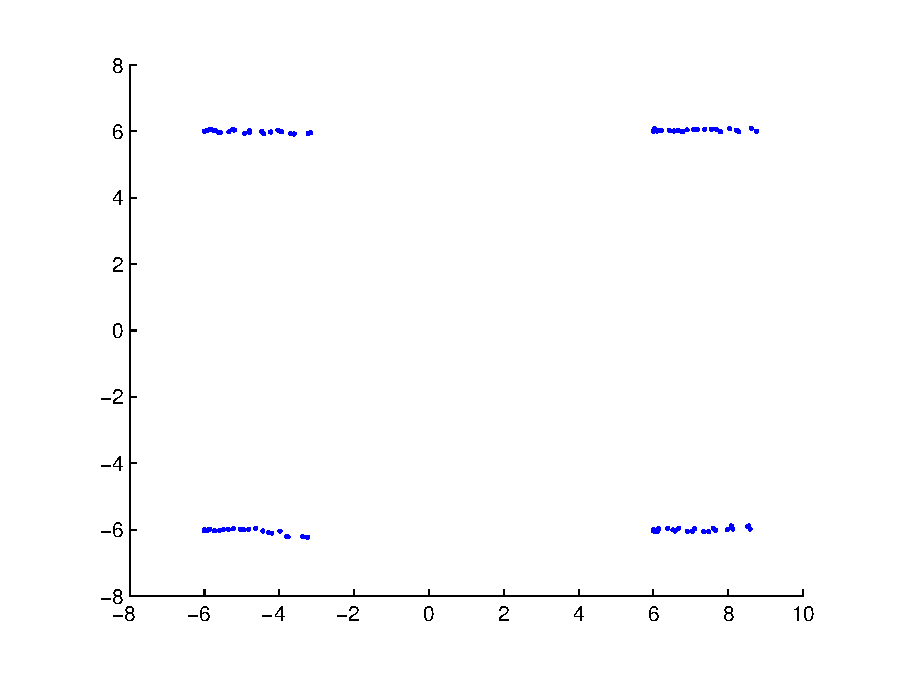
\includegraphics[width=7.5cm]{xmove.eps}
\caption{Movement along x axis}
\label{xmove}
\end{figure}

\item Moving along a random straight line. Similar to the movement along x axis. 
\begin{figure}[hb]
\centering
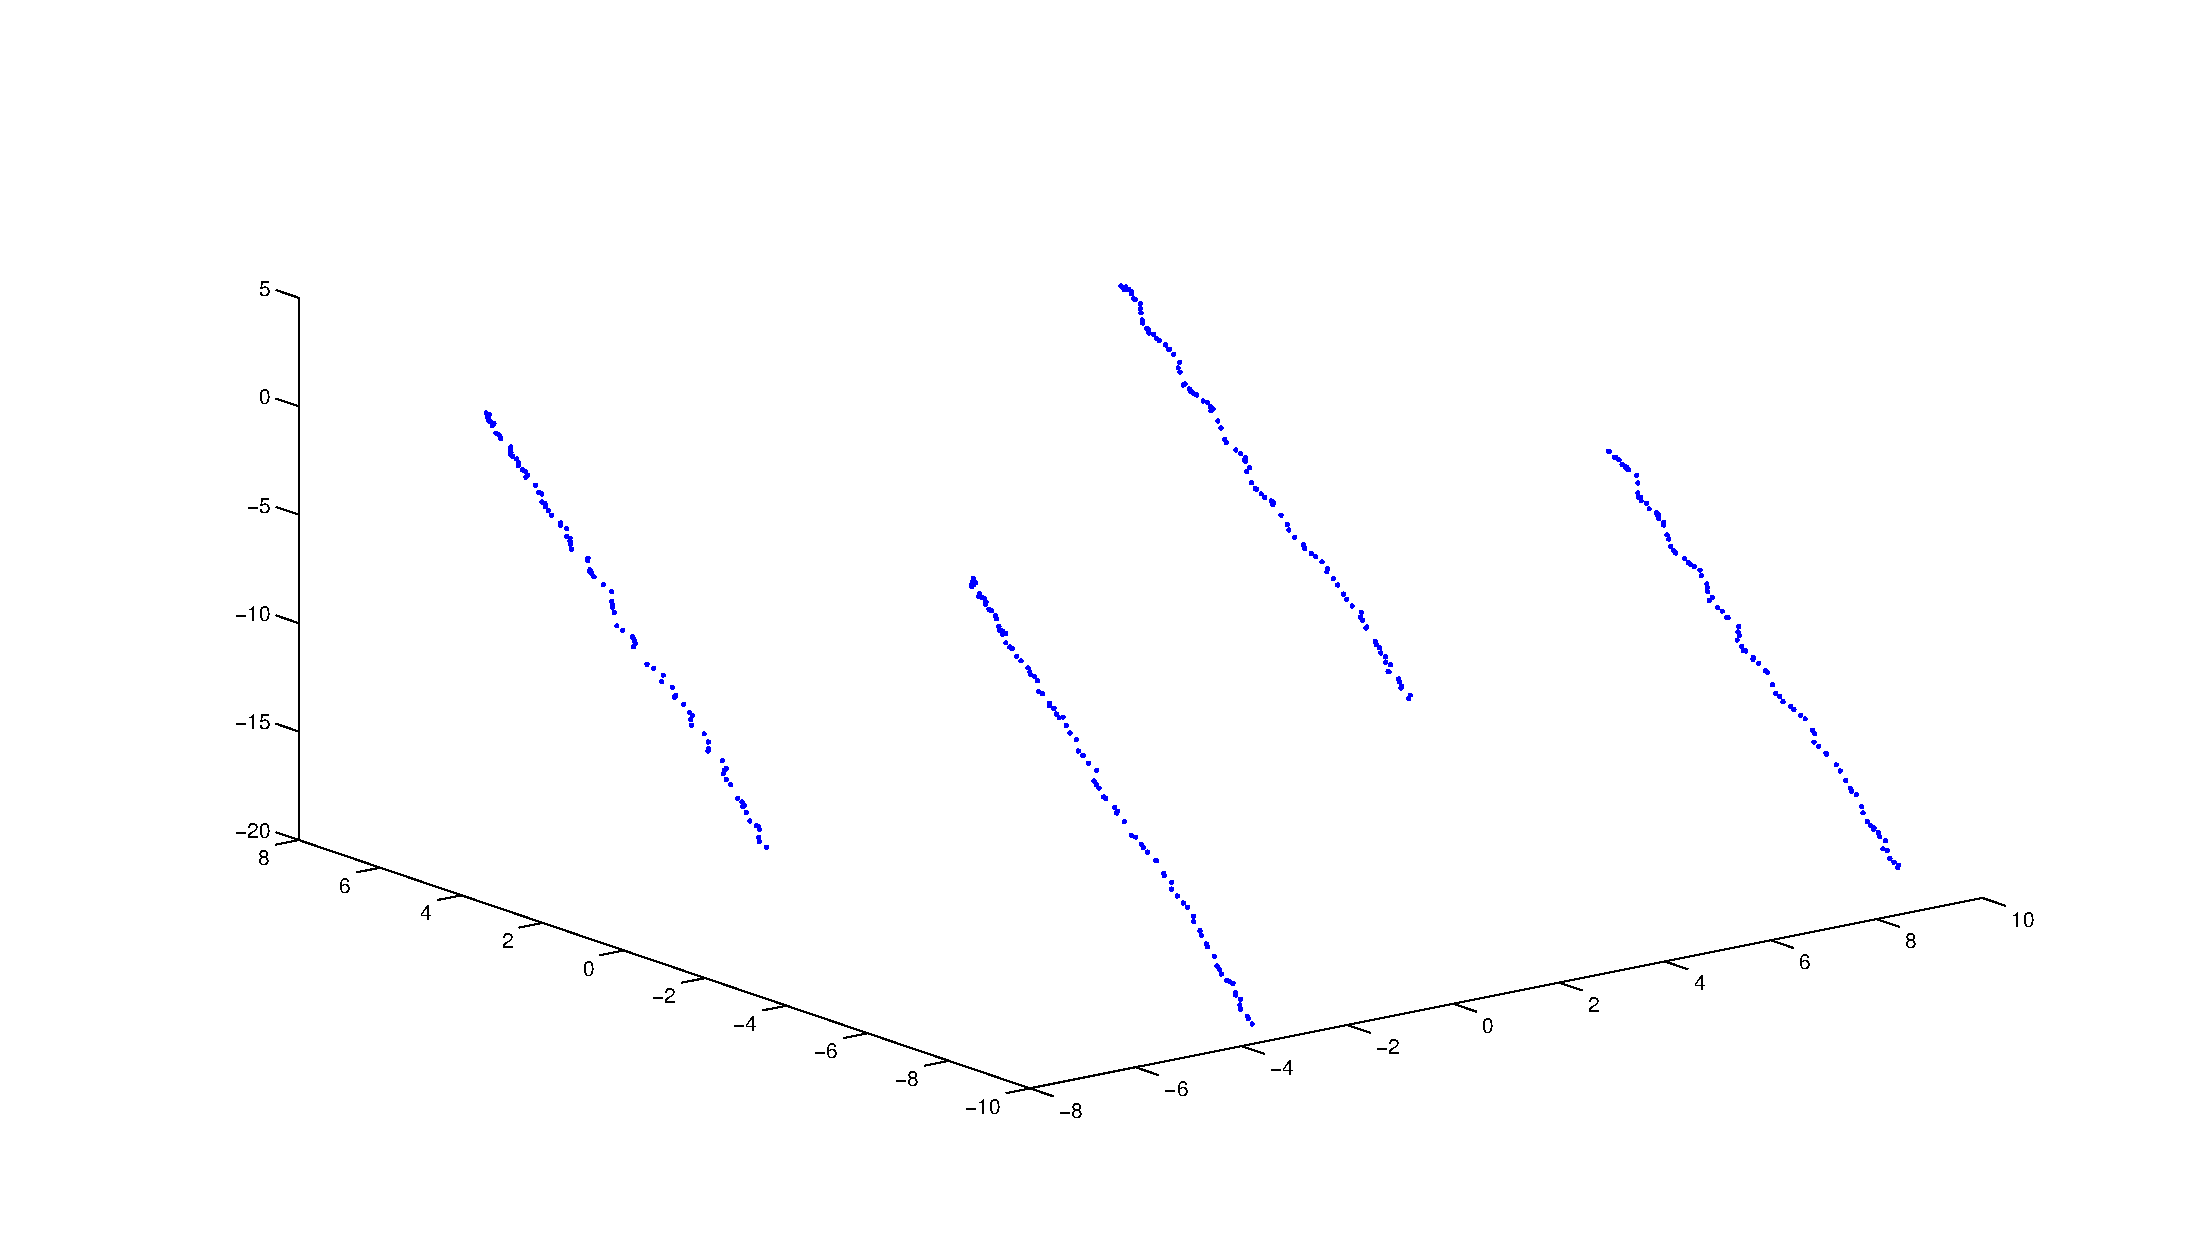
\includegraphics[width=7.5cm]{straightMove.eps}
\caption{Movement along a random straight line}
\label{straight}
\end{figure}

\item "Jump". Note that in this case, few error points occur. We repeat this experiment and find that these error are caused by LED signal missing during the movement. In our implementation, when some LEDs are not visible, we will take use the previous data of this LED. However, if the LED becomes invisible in one view for a long time and can be visible in another view, than the point pair matching may not works correctly as the previous data can be to old to generate a small energy when is calculating the distance to the correspondant epipolar line. It may leads to a chain effect to mistake other points' pair matching. The non-symmetric availablity of data in two cameras are one unsovled issue in our method. We leave this problem for our future work.

\begin{figure}
\centering
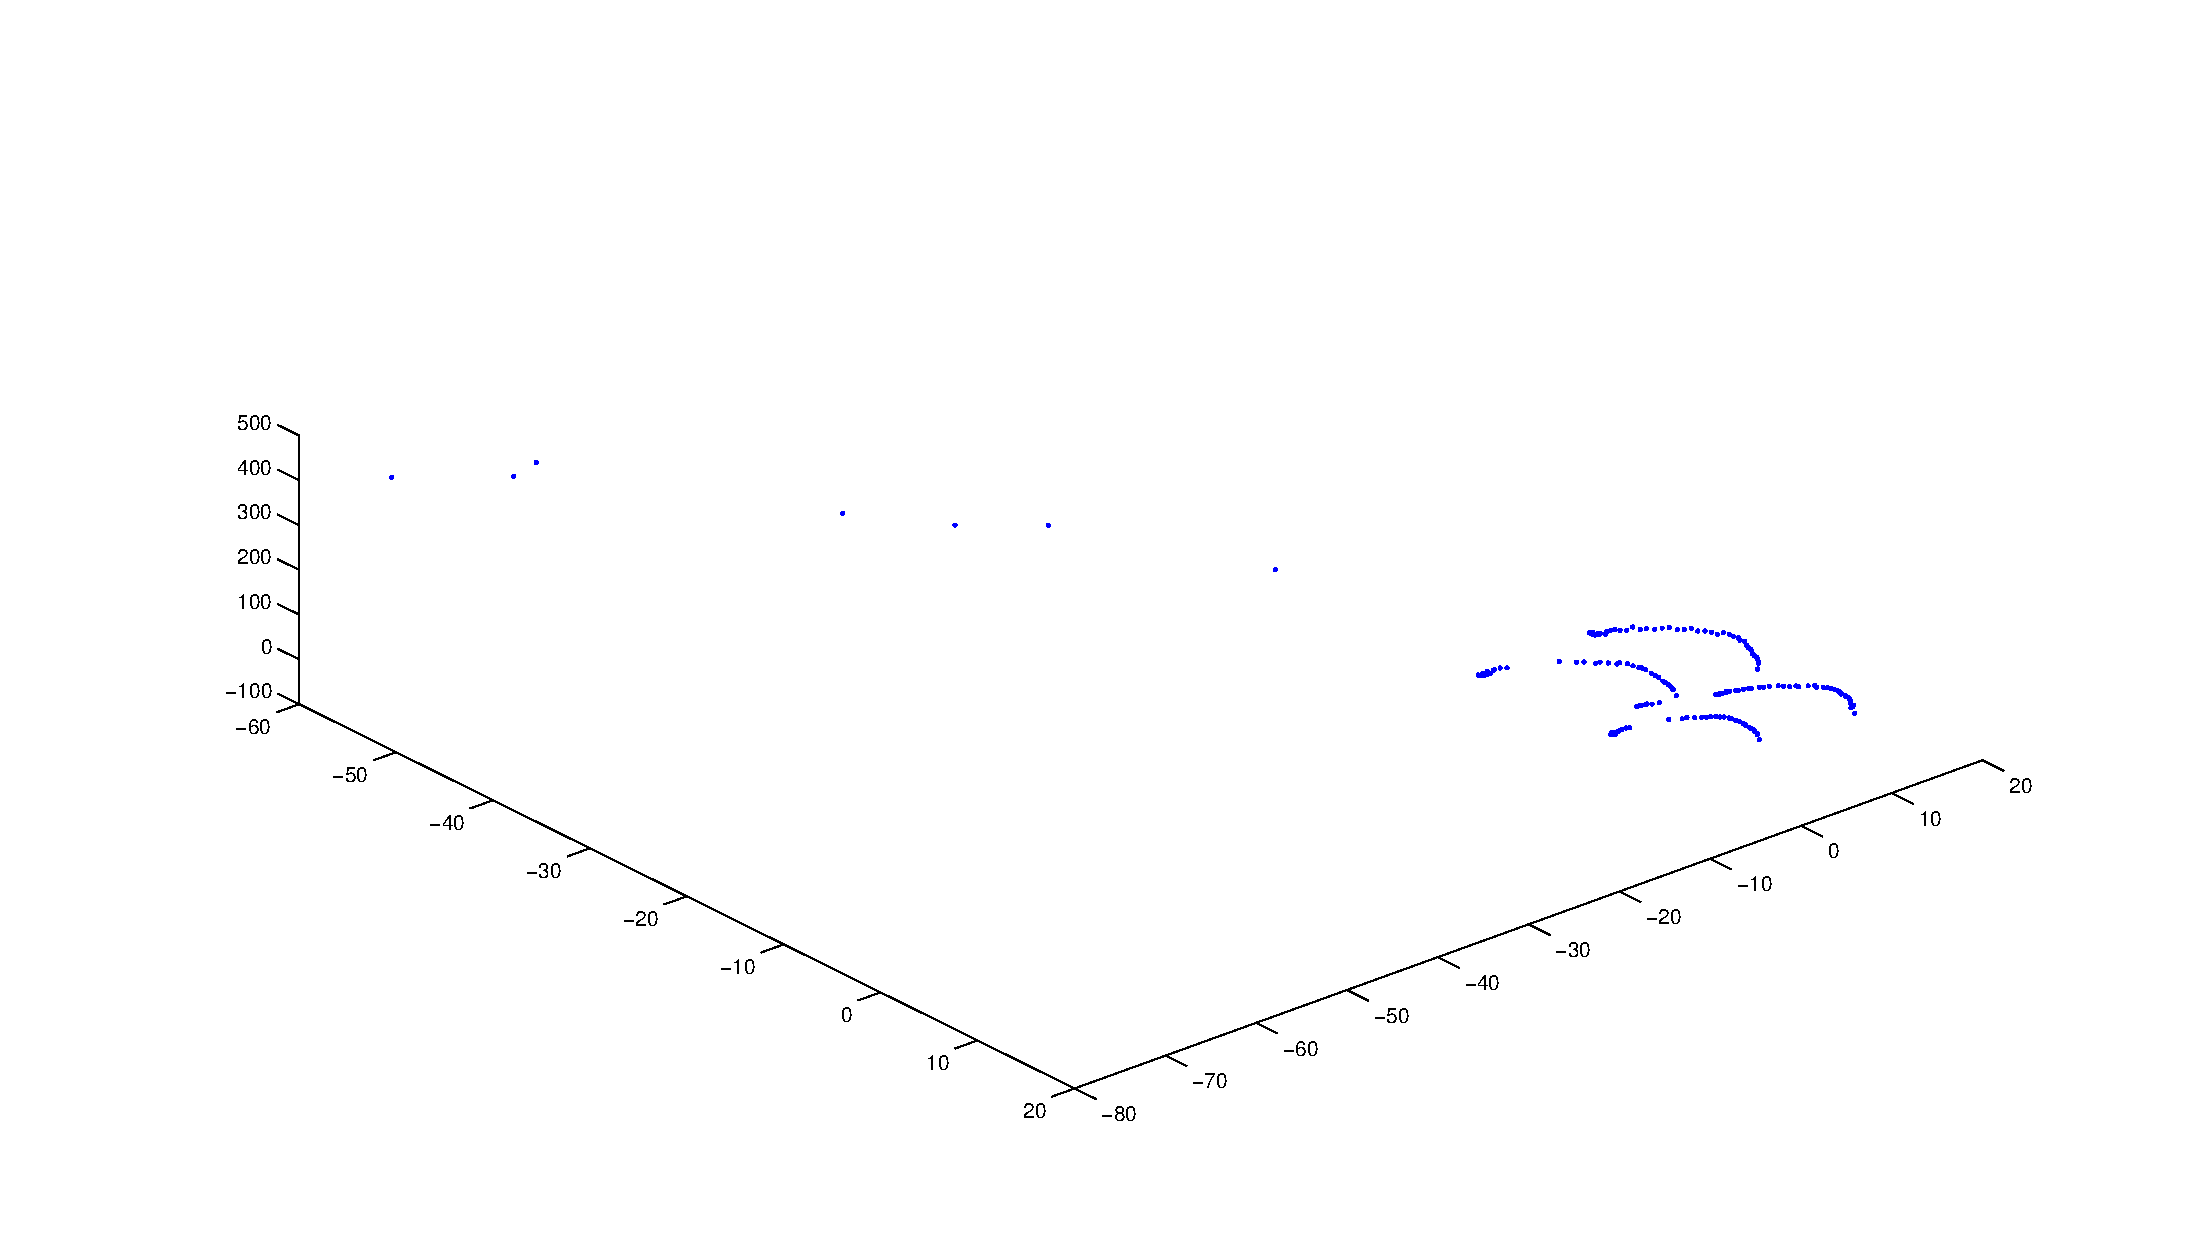
\includegraphics[width=7.5cm]{jump.eps}
\caption{Movement along a jumping curve}
\label{jump}
\end{figure}
\end{itemize}

%-------------------------------------------------------------------------
\section{Conclusion}


{\small
\bibliography{egbib}
\bibliographystyle{ieee}
}

%-------------------------------------------------------------------------
\end{document}
